% ============ §5.2 问题二 ============
\subsection{问题二：变物性双向热湿耦合模型}

\subsubsection{变物性与双向耦合}

整个烘干过程（预热平衡 + 恒温干燥）采用附录 3 的经验公式：$\rho,c_p,k$
依赖含水率 $C$，扩散系数 $D$ 同时依赖 $C$ 与温度 $T$：

\begin{equation}
\rho=650+128C,\qquad c_p=1450+2736\frac{C}{C+1},\qquad k=0.21+0.38\frac{C}{C+1}
\end{equation}
\begin{equation}
D=2.4\times10^{-3}e^{-0.45/C}e^{-3850/T_K}
\end{equation}

（$T_K$ 取开尔文）。耦合在整个求解域内双向进行：含水率 $C$ 通过
$\rho,c_p,k$ 改变热惯性与导热能力；温度 $T$ 通过 Arrhenius 项
$e^{-3850/T_K}$ 改变水分迁移速率。控制方程为

\begin{equation}
\rho(C)c_p(C)\frac{\partial T}{\partial t}=\frac{1}{r}\frac{\partial}{\partial r}\left(r k(C)\frac{\partial T}{\partial r}\right),\qquad
\frac{\partial C}{\partial t}=\frac{1}{r}\frac{\partial}{\partial r}\left(r D(C,T)\frac{\partial C}{\partial r}\right)
\end{equation}

边界条件与问题一相同（$h=25$ W/(m$^2$·K)、$\beta=8\times10^{-7}$ m/s），
环境条件两段拼接：0--4 h 用 5.1.1 的辨识模型，$t>4$ h 用平台外推值。

其中扩散系数的变化范围决定了问题的数值性质：$D$ 在 $C=2.55$、
$T=50$\,°C 时约 $1.3\times10^{-8}$ m$^2$/s，含水率降至 0.05 时约
$10^{-12}$ m$^2$/s——下降约 \textbf{4 个数量级}。干燥由此进入减速段：表面在约
12 h 即接近环境平衡值，而中心含水率的下降持续近 3 天。

\subsubsection{耦合求解与空间收敛}

数值求解沿用 5.1.3 的统一离散：两个场的内部节点拼接为
$\mathbf{y}=[\mathbf{T};\mathbf{C}]$（$2(N-1)$ 维），轴心与表面边界条件在
每次右端求值中由对称条件与 Robin 条件联立解出，时间积分用自适应隐式 BDF
（相对容差 $10^{-8}$，积分 72 h）。

空间分辨率是本问的关键数值问题。$N=48$ 时末位谱系数 $1.3\times10^{-3}$，
72 h 中心含水率 $0.1515$，与独立有限体积法参考解（$0.1380$）偏差
$0.0135$——干燥锋面未被充分分辨。加密后：

\begin{table}[H]
\centering
\caption{谱模式数收敛（72 h 中心含水率）}
\label{tab:conv}
\begin{tabular}{cccc}
\toprule
$N$ & 48 & 96 & 128 \\
\midrule
中心含水率 @72h & 0.1515 & 0.1386 & 0.1379 \\
末位谱系数 & $1.3\times10^{-3}$ & $6.8\times10^{-5}$ & $1.2\times10^{-5}$ \\
\bottomrule
\end{tabular}
\end{table}

$N=96$ 起与有限体积法一致到 \textbf{$6\times10^{-4}$}，$N=128$ 进一步收敛
（图~\ref{fig:conv}）。本文全部提交结果取 $N=128$；问题一剖面光滑，
$N=48$ 已足够（末位系数 $5\times10^{-13}$）。

\begin{figure}[H]
\centering
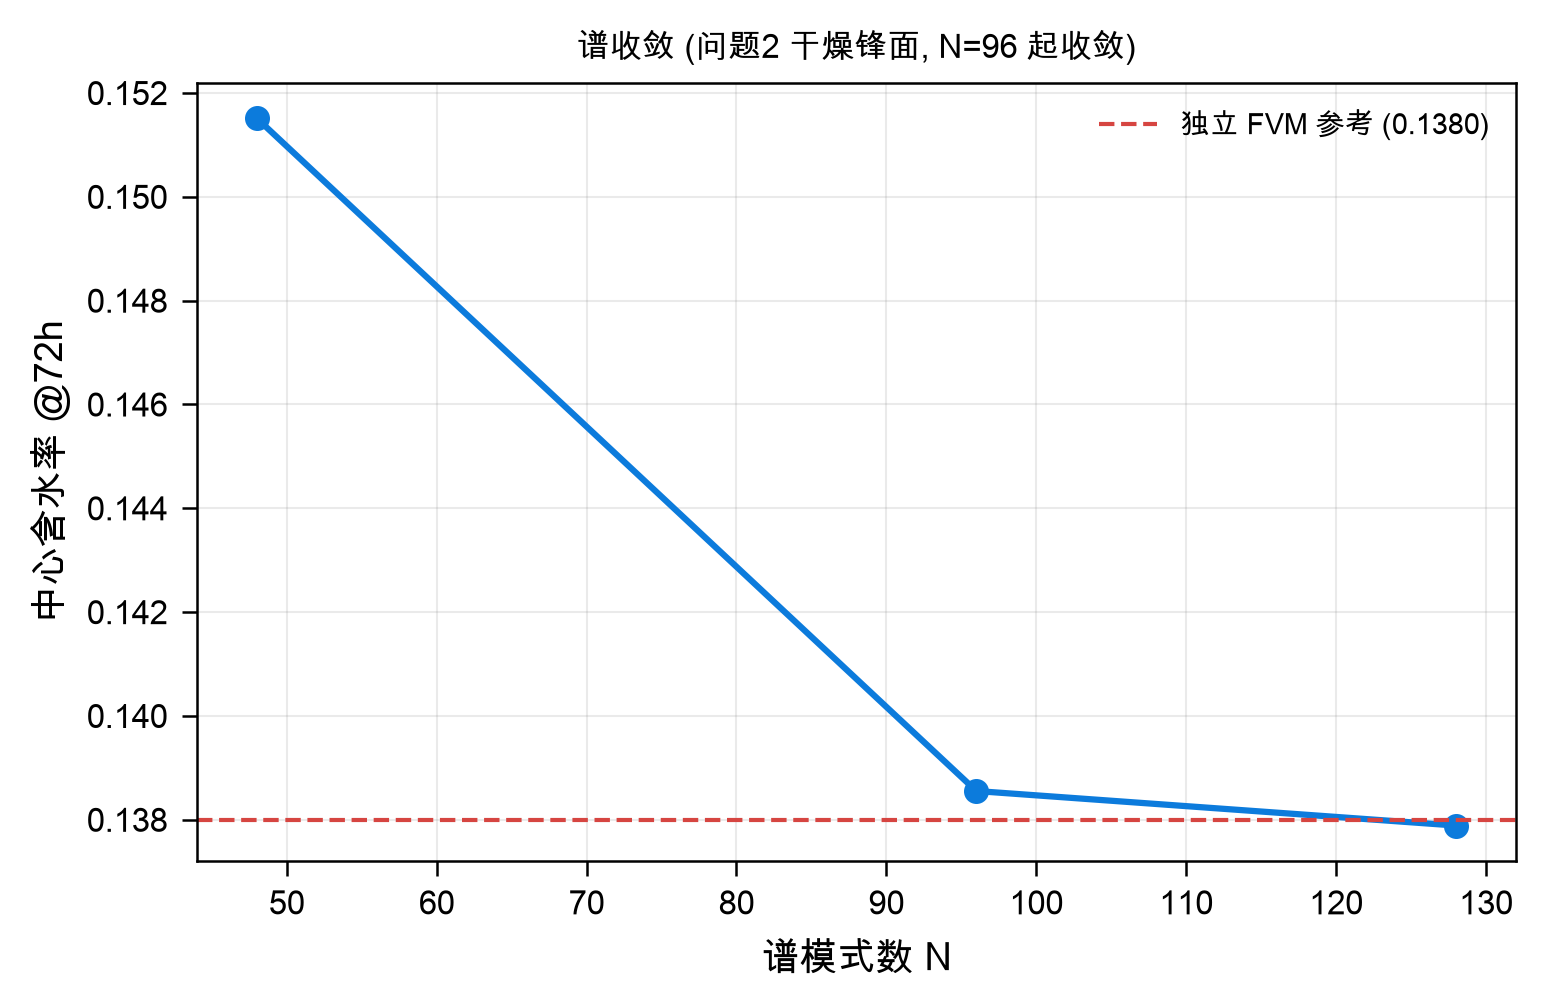
\includegraphics[width=0.62\textwidth]{fig11_convergence.png}
\caption{空间收敛：72 h 中心含水率随谱模式数的变化。$N=48$ 欠分辨，
$N=96$ 起与独立有限体积法参考解（虚线）一致。}
\label{fig:conv}
\end{figure}

\subsubsection{结果与讨论}

表~\ref{tab:q2t}、\ref{tab:q2c}（分别按题目表 3、表 4 格式输出，完整数据
见 result2.xlsx）：3 h 时温度场已均匀（表面 49.97\,°C、中心 49.85\,°C），
表面含水率降至 1.008 kg/kg、中心 1.766 kg/kg。图~\ref{fig:gamma} 给出
时间尺度比 $\Gamma=\alpha/D$ 的时空分布：湿态约 10，干态升至 $10^5$。
$\Gamma$ 小时热、湿两场的时间尺度接近；$\Gamma$ 大时温度场相对水分场
快速趋于准稳态，总干燥过程逐渐受水分扩散控制。这与 6.2 节中烘干时长对
换热系数不敏感的结果一致。

\begin{table}[H]
\centering
\caption{3 小时内药材的温度（按题目表 3 的格式要求输出，单位 °C）}
\label{tab:q2t}
\begin{tabular}{c|ccccc}
\toprule
时间/h & 0 cm & 0.5 cm & 1 cm & 1.5 cm & 2 cm \\
\midrule
0.5 & 32.1896 & 32.3824 & 32.9661 & 33.9610 & 35.4133 \\
1.0 & 40.3821 & 40.5541 & 41.0610 & 41.8784 & 42.9990 \\
1.5 & 45.8471 & 45.9352 & 46.1932 & 46.6055 & 47.1395 \\
2.0 & 48.4504 & 48.4882 & 48.5985 & 48.7736 & 49.0032 \\
2.5 & 49.4670 & 49.4793 & 49.5137 & 49.5646 & 49.6618 \\
3.0 & 49.8494 & 49.8553 & 49.8746 & 49.9101 & 49.9667 \\
\bottomrule
\end{tabular}
\end{table}

\begin{table}[H]
\centering
\caption{3 小时内药材的水分浓度（按题目表 4 的格式要求输出，单位 kg/kg）}
\label{tab:q2c}
\begin{tabular}{c|ccccc}
\toprule
时间/h & 0 cm & 0.5 cm & 1 cm & 1.5 cm & 2 cm \\
\midrule
0.5 & 2.5499 & 2.5489 & 2.5256 & 2.3257 & 1.6486 \\
1.0 & 2.5257 & 2.4948 & 2.3578 & 2.0230 & 1.4711 \\
1.5 & 2.3861 & 2.3256 & 2.1344 & 1.8020 & 1.3476 \\
2.0 & 2.1708 & 2.1084 & 1.9236 & 1.6259 & 1.2311 \\
2.5 & 1.9566 & 1.9006 & 1.7360 & 1.4720 & 1.1166 \\
3.0 & 1.7662 & 1.7165 & 1.5702 & 1.3333 & 1.0081 \\
\bottomrule
\end{tabular}
\end{table}


\begin{figure}[H]
\centering
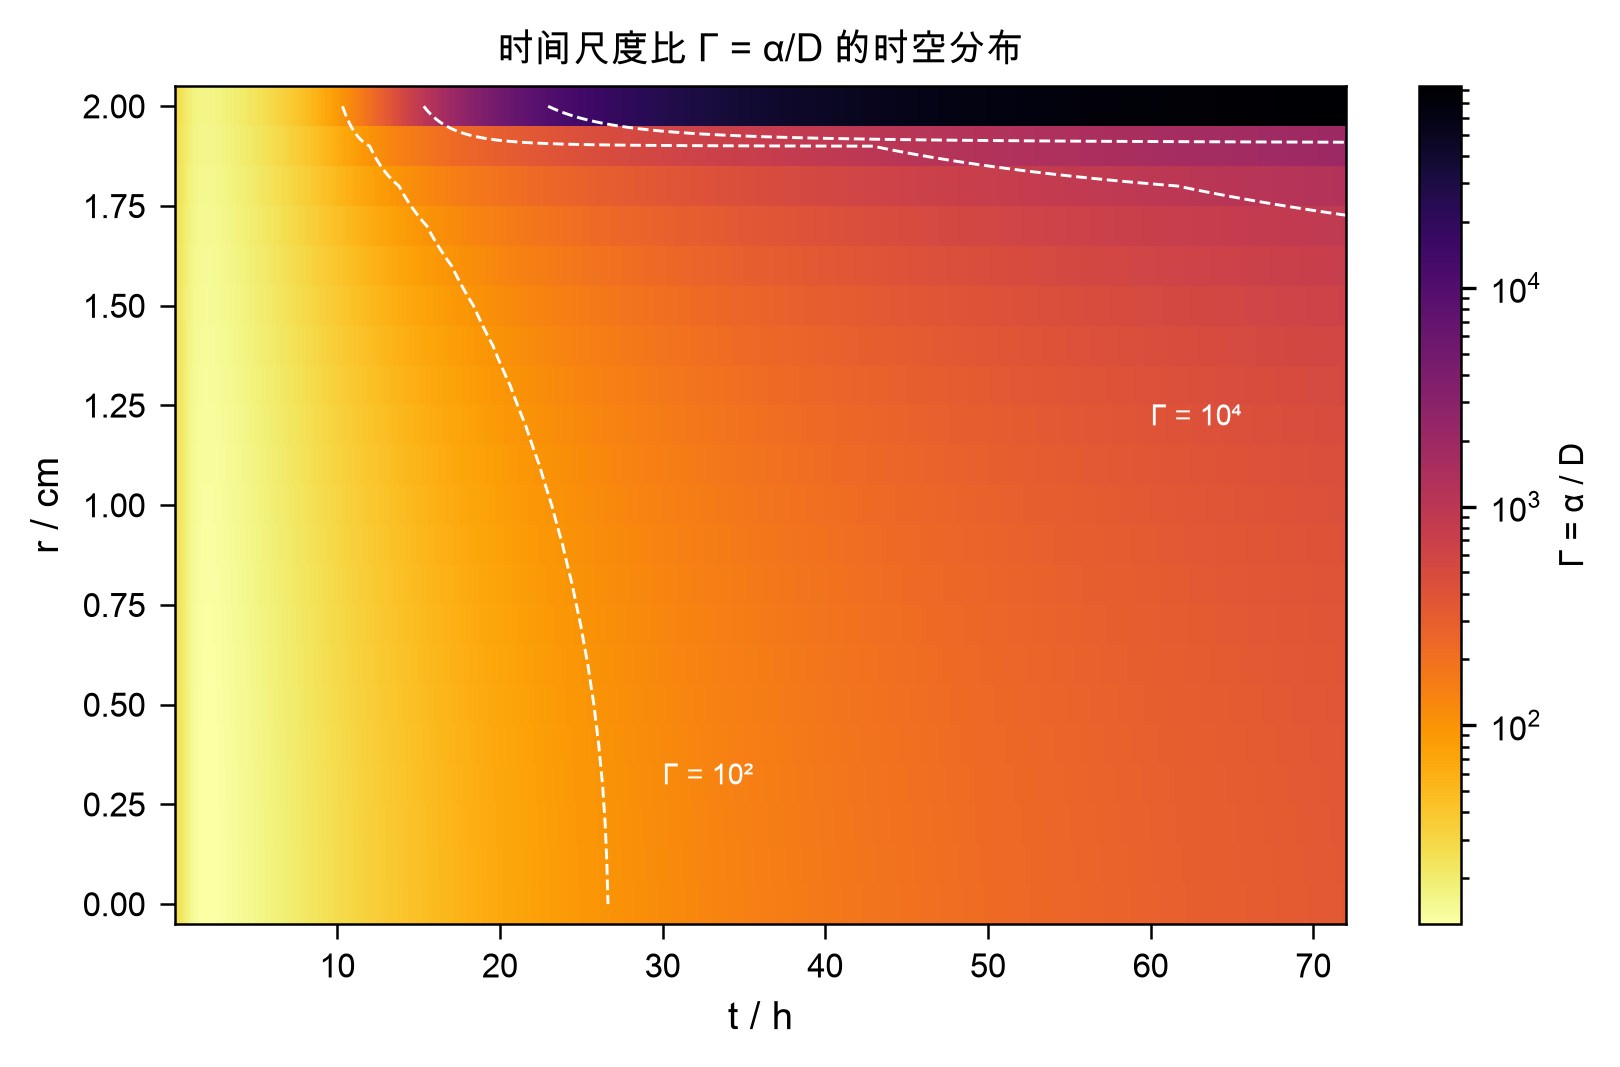
\includegraphics[width=0.62\textwidth]{fig5_lu.png}
\caption{时间尺度比 $\Gamma=\alpha/D$ 的时空分布（对数色标）。$\Gamma$ 增大
表示热扩散相对水分扩散更快，温度场更快趋于准稳态。}
\label{fig:gamma}
\end{figure}

% ============ §5.3 问题三 ============
\subsection{问题三：烘干时长判定}

烘干要求药材各处水分浓度低于 0.15 kg/kg。定义
\begin{equation}
C_{\max}(t)=\max_{0\le r\le R}C(r,t)
\end{equation}
程序在问题二的解上以 60 s 分辨率对 $C_{\max}(t)$ 做实际扫描（输出网格
21 个径向点取最大值），寻找首个满足 $C_{\max}(t)<0.15$ 的时刻：

\begin{equation}
t_{end}=208200\ \mathrm{s}=\mathbf{57.83\ h}
\end{equation}

数值解在全部输出时刻均保持由中心向表面单调下降（逐时刻检查通过），
$C_{\max}$ 始终出现在 $r=0$ 处，因此后续分析与图表等价地监测
$C(0,t)$。跨越细节：$t=208140$ s 时中心含水率 $0.150002$，$t=208200$ s 时
$0.149983$（图~\ref{fig:criterion}）。需要注意，跨越处中心曲线衰减速率仅
约 $10^{-3}$ /h，判据对数值精度敏感：本文谱配点（$N=128$）给出 57.83 h，
独立有限体积法（400 节点、800 节点验证）给出 57.77 h，两种独立离散
相差 \textbf{0.06 h}。这一敏感性在表~\ref{tab:q3} 的最后一行体现为恰好跨过判据
的数值。

\begin{figure}[H]
\centering

\includegraphics[width=0.95\textwidth]{fig8_criterion.png}
\caption{中心/表面含水率轨迹与 0.15 判据线（内嵌 56.5--60.5 h 放大图）。}
\label{fig:criterion}
\end{figure}

\begin{figure}[H]
\centering

\includegraphics[width=0.95\textwidth]{fig4_front.png}
\caption{全流程水分浓度二维热图（左）与干燥锋面位置随时间的变化
（右，虚线为 $\sqrt{t}$ 参考）。}
\label{fig:front}
\end{figure}

与附件 2 的半径收缩平台（约 70 h）比较，57.83 h 与之处于同一物理量级
（收缩阶段含水率已很低，两种现象的时间尺度自洽），不构成对烘干时长的
独立定量验证。

\begin{table}[H]
\centering
\caption{药材烘干过程的水分浓度（按题目表 5 的格式要求输出，单位 kg/kg；末行为判据跨越时刻）}
\label{tab:q3}
\begin{tabular}{c|ccccc}
\toprule
时间/h & 0 cm & 0.5 cm & 1 cm & 1.5 cm & 2 cm \\
\midrule
6 & 1.0172 & 0.9884 & 0.9017 & 0.7550 & 0.5326 \\
12 & 0.4564 & 0.4434 & 0.4032 & 0.3298 & 0.1640 \\
18 & 0.2990 & 0.2917 & 0.2688 & 0.2254 & 0.0844 \\
24 & 0.2380 & 0.2329 & 0.2168 & 0.1856 & 0.0663 \\
30 & 0.2063 & 0.2020 & 0.1892 & 0.1642 & 0.0597 \\
36 & 0.1865 & 0.1827 & 0.1718 & 0.1505 & 0.0565 \\
42 & 0.1727 & 0.1693 & 0.1597 & 0.1408 & 0.0547 \\
48 & 0.1623 & 0.1593 & 0.1507 & 0.1335 & 0.0536 \\
54 & 0.1543 & 0.1516 & 0.1437 & 0.1278 & 0.0529 \\
57.83 & 0.1500 & 0.1474 & 0.1399 & 0.1247 & 0.0525 \\
\bottomrule
\end{tabular}
\end{table}


% ============ §5.4 问题四 ============
\subsection{问题四：随体坐标下干基含水率守恒方程}

\subsubsection{干基含水率的物质守恒}

问题四中半径随失水收缩，$R(t)$ 由附件 2 给定（2.00$\to$1.198 cm，保形
三次样条插值，$t>252000$ s 平台外推）。收缩使求解域随时间变化，直接在内
部固定网格上离散需要处理移动边界两侧的守恒关系。本文改用随体坐标
（网格随材料一起运动），利用干基含水率的定义简化方程。

干基含水率 $C=m_w/m_s$ 依附于干物质：固定一组随体坐标，就固定了一团
干物质，其质量 $m_s$ 不随时间变化。设材料速度 $u=\dot R\,r/R$（径向
仿射收缩），干物质密度 $\rho_s\propto1/R^2$ 均匀压实，水分守恒的欧拉
形式为

\begin{equation}
\frac{\partial(\rho_s C)}{\partial t}+\nabla\cdot(u\,\rho_s C)=\nabla\cdot(\rho_s D\nabla C)
\end{equation}

将 $\rho_s$ 与 $u$ 的表达式代入并变换到随体坐标，对流项、体积膨胀项与
密度变化项相互消去（推导见附录 A），得到

\begin{equation}
\left.\frac{\partial C}{\partial t}\right|_{g}=\frac{1}{r}\frac{\partial}{\partial r}\left(rD(C,T)\frac{\partial C}{\partial r}\right)
\end{equation}

即：在随体坐标下，干基含水率的演化仅由相对扩散决定。一个直接的检验是
均匀场情形：$C$ 为常数时方程右端恒为零，含水率保持不变——收缩本身不会
产生虚假的含水率变化。这也说明径向仿射收缩是本文的\textbf{关键假设}：题目只提供
$R(t)$ 的径向数据，各向异性或轴向收缩未建模。

物性换为附录 4（$\rho=760+90C$、$c_p=1850+2150C/(C+1)$、
$k=0.12+0.20C/(C+1)$、$D=4.2\times10^{-4}e^{-0.30/C}e^{-3850/T_K}$），
温度方程同构。数值实现：随体网格的微分矩阵按 $R(t)$ 逐次更新，边界条件
求解与 5.2.2 相同，$N=96$、相对容差 $10^{-8}$。

\subsubsection{结果与控制变量分解}

问题四的设置相对问题三同时改变了两件事：物性体系（附录 3 $\to$ 附录 4）与
求解域（固定半径 $\to$ 收缩）。二者对烘干时长的影响方向相反，直接比较
两个问题的时间差无法将全部差异归因于收缩。为此增设一个控制变量基准：

\begin{table}[H]
\centering
\caption{问题四的对照设置与烘干时长（判据 $C_{\max}<0.15$）}
\label{tab:control}
\begin{tabular}{lccc}
\toprule
设置 & 物性 & 半径 & 烘干时长 \\
\midrule
问题三 & 附录 3 & $R=2$ cm 固定 & 57.83 h \\
基准 A（本文增设） & 附录 4 & $R=2$ cm 固定 & $>150$ h（模拟至 150 h 仍未达标） \\
模型 B（问题四） & 附录 4 & 附件 2 $R(t)$ & 51.15 h \\
\bottomrule
\end{tabular}
\end{table}

据此把问题三到问题四的总差异分解为两部分：
\begin{equation}
\Delta t_{total}=57.83-51.15=6.68\ \mathrm{h}
=\underbrace{\Delta t_{props}}_{\text{物性体系}}+\underbrace{\Delta t_{shrink}}_{\text{纯几何收缩}}
\end{equation}
其中 $\Delta t_{props}=t_{Q3}-t_{A}<0$（附录 4 的扩散系数在湿态约为附录 3
的五分之一，物性变化使干燥变慢，幅度超过 92 h），
$\Delta t_{shrink}=t_{A}-t_{B}>98.85$ h（收缩使扩散路径缩短，加速幅度
超过 98 h，即相对基准 A 缩短约三分之二）。两重效应相互抵消后净得 6.68 h。
**若仅比较问题三与问题四的总差异，会严重低估收缩的加速作用。**

\begin{figure}[H]
\centering

\includegraphics[width=0.95\textwidth]{fig9_shrink.png}
\caption{（a）附件 2 实测半径与插值轨迹；（b）三种设置的中心含水率对比
（问题三 / 附录 4 固定半径 / 附录 4 收缩）；（c）收缩--失水关系。}
\label{fig:shrink}
\end{figure}

\begin{table}[H]
\centering
\caption{药材烘干过程的水分浓度（表 6, 收缩模型, kg/kg; 末列为药材表面处的值, 最后一列为该时刻的半径）}
\begin{tabular}{c|ccccc}
\toprule
时间/h & 0 cm & 0.5 cm & 1.0 cm & 药材表面 & $R(t)$/cm \\
\midrule
6 & 1.7192 & 1.5374 & 1.0223 & 0.4202 & 1.374 \\
12 & 0.7379 & 0.6548 & 0.4084 & 0.1668 & 1.248 \\
18 & 0.4090 & 0.3689 & 0.2398 & 0.0891 & 1.214 \\
24 & 0.2853 & 0.2612 & 0.1791 & 0.0672 & 1.204 \\
30 & 0.2265 & 0.2095 & 0.1493 & 0.0594 & 1.201 \\
36 & 0.1929 & 0.1798 & 0.1317 & 0.0558 & 1.200 \\
42 & 0.1713 & 0.1605 & 0.1200 & 0.0540 & 1.200 \\
48 & 0.1562 & 0.1469 & 0.1116 & 0.0529 & 1.200 \\
51.15 & 0.1500 & 0.1412 & 0.1080 & 0.0525 & 1.200 \\
\bottomrule
\end{tabular}
\end{table}

